
\begin{enumerate}[\bfseries \mbox{Ejercicio} 1.]

%-------------------- 1.
\item \textbf{\boldmath Dados los  vectores $\vec{a},\vec{b},\vec{c}$ que satisfacen la condición $\vec{a}+\vec{b}+\vec{c}=\vec{0}$ y sabiendo que $\|\vec{a}\|=3,\|\vec{b}\|=1,\|\vec{c}\|=4.$ Calcular $\vec{a}\circ \vec{b}+\vec{b}\circ \vec{c}+\vec{a}\circ \vec{c}$.\\\\
    Respuesta.-}\; Sea $\vec{a}+\vec{b}+\vec{c}=\vec{0}$. Entonces, por propiedades de producto escalar y modulo
    $$\begin{array}{rcl}
	\vec{0}=\|\vec{a}+\vec{b}+\vec{c}\|^2 &=& \|\vec{a}+(\vec{b}+\vec{c})\|^2\\
				      &=& \|\vec{a}\|^2+2[\vec{a}\circ(\vec{b}+\vec{c})]+\|\vec{b}+\vec{c}\|^2\\
				      &=& \|\vec{a}\|^2+2\vec{a}\circ \vec{b}+2\vec{a}\circ \vec{b}+\|\vec{b}\|^2+2\vec{b}\circ \vec{c}+\|\vec{c}\|^2\\
				      &=& \|\vec{a}\|^2 + \|\vec{b}\|^2 + \|\vec{c}\|^2 + 2(\vec{a}\circ \vec{b} + \vec{a}\circ \vec{c} + \vec{b}\circ \vec{c}) 
    \end{array}$$
    Por lo tanto,
    $$\vec{a}\circ \vec{b} + \vec{a}\circ \vec{c} + \vec{b}\circ \vec{c} = -\dfrac{\|\vec{a}\|^2 + \|\vec{b}\|^2 + \|\vec{c}\|^2}{2} = -\dfrac{3^2+1^2+4^2}{2}=-13.$$\\

%-------------------- 2.
\item \textbf{Demostrar que las diagonales de un rombo son ortogonales entre si.\\\\
    Demostración.-}\; Sean $\vec{a},\vec{b},\vec{c},\vec{d},\vec{e},\vec{f}\in V_n $. De donde gráficamente se tiene:
	    \begin{center}
		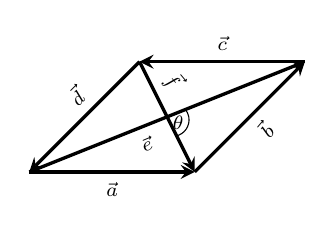
\begin{tikzpicture}[scale=.7]
		  \tikzstyle{every node}=[font=\scriptsize]
		  \draw[line width=1.2pt,-stealth](0,0)--(3,0) node[rotate=0,pos=0.5,below]{$\vec{a}$};
		  \draw[line width=1.2pt,-stealth](3,0)--(5,2) node[rotate=50,pos=0.5, below]{$\vec{b}$};
		  \draw[line width=1.2pt,-stealth](5,2)--(2,2) node[rotate=0,pos=0.5, above]{$\vec{c}$};
		  \draw[line width=1.2pt,-stealth](2,2)--(0,0) node[rotate=45,pos=0.45, above]{$\vec{d}$};
		  \draw[line width=1.2pt,-stealth](0,0)--(5,2) node[rotate=23,pos=0.4, below]{$\vec{e}$};
		  \draw[line width=1.2pt,-stealth](2,2)--(3,0) node[rotate=-50,pos=0.3, above]{$\vec{f}$};
		  \draw(2.65,.65) arc (-80:40:.3);
		  \draw(2.7,.9)node[]{$\theta$};
		\end{tikzpicture}
	    \end{center}
	    Así,  $$\cos (\theta) = \dfrac{\vec{e}\circ \vec{f}}{\|\vec{e}\|\|\vec{f}\|} \quad \Rightarrow \quad \theta = \cos^{-1}\left[\dfrac{ (\vec{a}+\vec{b})\circ(\vec{d}+\vec{a})}{\|\vec{e}\|\|\vec{f}\|}\right].$$

	    Luego, ya que $\vec{a},\vec{b},\vec{c},\vec{d}$ forman un rombo. Es decir, un paralelogramo de lados iguales, entonces $\vec{d}=-\vec{b}$, por lo que:
	    $$\theta = \cos^{-1}\left[\dfrac{(\vec{a}+\vec{b})\circ(-\vec{b}+\vec{a})}{\|\vec{e}\|\|\vec{f}\|}\right].$$

	    Por las propiedades de producto interno y $\|\vec{a}\|=\|\vec{b}\|$,

	    $$\begin{array}{rcl}
		\theta&=&\cos^{-1}\left[\dfrac{\vec{a}\circ (-\vec{b})+ \vec{b}\circ(-\vec{b})+ \vec{a}\circ \vec{a}+ \vec{b}\circ \vec{a}}{\|\vec{e}\|\|\vec{f}\|}\right]\\\\
		      &=&\cos^{-1}\left[\dfrac{-(\vec{a}\circ \vec{b})- (\vec{b}\circ \vec{b}) + \vec{a}\circ \vec{a}+ \vec{a}\circ \vec{b}}{\|\vec{e}\|\|\vec{f}\|}\right]\\\\
		      &=&\cos^{-1}\left(\dfrac{ \vec{a}\circ \vec{a}- \vec{b}\circ \vec{b}}{\|\vec{e}\|\|\vec{f}\|}\right)=\cos^{-1}\left(\dfrac{\|\vec{a}\|^2-\|\vec{b}\|^2}{\|\vec{e}\|\|\vec{f}\|}\right)\\\\
		      &=& \cos^{-1}\left(\dfrac{0}{\|\vec{e}\|\|\vec{f}\|}\right) = \dfrac{\pi}{2}.\\\\
	    \end{array}$$
	    Por lo tanto,
	    $$\vec{e}\perp \vec{f}.$$\\


%-------------------- 3.
\item \textbf{\boldmath Encontrar la ecuación del plano que pasa por $(-1,4,2)$ y que contiene a la recta de intersección de los planos.
    $$4x-y+z-2=0 \qquad \mbox{y}\qquad 2x+y-2z-3=0.$$\\
    Respuesta.-}\; La ecuación del plano que pasa por la línea de intersección de los planos: $4x-y+z-2=0$ y $2x+y-2z-3=0$ está dada por:
    $$4x-y+z-2+\lambda(2x+y-2z-3)=0$$
    Dado que el plano anterior pasa por el punto dado $(-1,4,2)$, satisfará la ecuación del plano $4x-y+z-2+\lambda(2x+y-2z-3)=0$ de la siguiente manera
    $$4(-1)-4+2-2+\lambda(2(-1)+4-2\cdot 2-3)=0 \quad \Rightarrow \quad \lambda =-\dfrac{8}{5}.$$
    Luego sustituyendo $\lambda$ en la ecuación del plano $4x-y+z-2+\lambda(2x+y-2z-3)=0$ se concluye que:
    $$4x-y+z-2-\dfrac{8}{5}(2x+y-2z-3)=0 \quad \Rightarrow \quad 4x-13y+21z+14=0.$$\\

%-------------------- 4.
\item \textbf{\boldmath Demostrar que la distancia $D$ entre los planos paralelos $ax+by+cz+d=d_1$ y $ax+by+cz+d=d_2$ está dada por:
$$D=\dfrac{|d_2-d_1|}{\sqrt{a^2+b^2+c^2}}.$$\\
    Demostración.-}\; Sabemos que  para $\mathscr{P}:ax+by+cz=d$ con $P_0=(x_0,y_0)$, la distancia está dada por:
    $$d(P_0,\mathscr{P})\dfrac{|ax_0,by_0+cz_0-d|}{\sqrt{a^2+b^2+c^2}}.$$
    Primero, hallemos un punto $P_0$ del plano $ax+by+cz+d=d_1$.
    $$\left\{\begin{array}{rcl}
	x&=&0\\
	y&=&0\\
\end{array}\right.\quad \Rightarrow \quad z=\dfrac{d_1-d}{c}.$$
Así $P_0=\left(0,0,\dfrac{d_1-d}{c}\right)$
Por último, hallemos $D=d(P_0,ax+by+cz+d=d_2)$ de la siguiente manera,
$$\begin{array}{rcl}
    D&=&\dfrac{|a\cdot 0+b\cdot 0 +c\left(\frac{d_1-d}{c}\right)-d_2+d|}{\sqrt{a^2+b^2+c^2}}\\\\
     &=&\dfrac{|d_1-d-d_2+d}{\sqrt{a^2+b^2+c^2}|}\\\\
     &=&\dfrac{|d_1-d_2|}{\sqrt{a^2+b^2+c^2}}.\\\\
\end{array}$$

\end{enumerate}
